\documentclass[12pt,a4paper]{article}
\usepackage[utf8]{inputenc}
\usepackage[T1]{fontenc}
\usepackage{amsmath}
\usepackage{amsfonts}
\usepackage{amssymb}
\usepackage{amsthm}
\usepackage{algorithm}           
\usepackage{algorithmic} 
\usepackage{graphicx}
\usepackage{subfigure}
\usepackage{float}
\renewcommand{\algorithmicrequire}{\textbf{Parameters:}} \renewcommand{\algorithmicensure}{\textbf{Iteration:}} 
\newtheorem*{lemma}{Lemma}
\newtheorem*{theorem}{Theorem}
\newtheorem*{prf}{\textbf{Proof}}
\usepackage{caption}
\DeclareMathOperator{\n}{\nabla}
\DeclareMathOperator{\E}{\mathrm{E}}
\DeclareMathOperator{\xyz}{\textbf{numpy.random.normal()}}
\title{CS331-HW6-Lukang-Sun}
\begin{document}
	\maketitle
	\begin{algorithm}
		\caption{DCGD-SHIFT}
		\label{alg:1}
		\begin{algorithmic}[1]
			\REQUIRE shift $h_i$,learning rate $\gamma>0$, starting point $x^{0} \in \mathbb{R}^{d}$, compression operators $\mathcal{C}_{1} \in \mathbb{B}^{d}\left(\omega_{1}\right), \ldots, \mathcal{C}_{n} \in \mathbb{B}^{d}\left(\omega_{n}\right),\mathcal{C}=Id$
			\FOR{$k=0,1,2, \ldots$ }
			\FOR{all workers $i \in\{1,2, \ldots, n\}$ in parallel}
			\STATE Compute local gradient $\nabla f_{i}\left(x^{k}\right)$
			\STATE Compress local gradient $g_{i}^{k}={C}_{i}^{k}\left(\nabla f_{i}\left(x^{k}\right)-h_i\right)$
			\STATE Send $g_{i}^{k}$ to master
			\ENDFOR
			\STATE Master computes the aggregate $\hat{g}^{k}=\frac{1}{n} \sum_{i=1}^{n} g_{i}^{k}+\frac{1}{n}\sum_{i=1}^nh_i$ 
			\STATE Master broadcasts the compressed aggregate $g^{k}=\mathcal{C}(\hat{g}^{k})$ to all workers
			\FOR {all workers $i \in\{1,2, \ldots, n\}$ in parallel}
			\STATE  Compute the next iterate $x^{k+1}=\operatorname{prox}_{\gamma R}\left(x^{k}-\gamma g^{k}\right)$
			\ENDFOR
			\ENDFOR
			
		\end{algorithmic}	 
	\end{algorithm}
	\paragraph{p1.}
	\begin{theorem}
	Assume $f_{i}$ is convex and $L_{i}$-smooth for all $i$, and let $f$ be L-smooth. Let the gradient estimator $\mathrm{g}$ be defined as in Algorithm \ref{alg:1}, where
	$$
	\mathcal{C}_{1} \in \mathbb{B}^{d}\left(\omega_{1}\right), \quad \mathcal{C}_{2} \in \mathbb{B}^{d}\left(\omega_{2}\right), \quad \ldots, \quad \mathcal{C}_{n} \in \mathbb{B}^{d}\left(\omega_{n}\right),\quad \mathcal{C} = Id
	$$
	are independent compression operators,$h_i=\nabla f_i(y)$ . Then
	$$
	G(x, y) \leq 2 A D_{f}(x, y)
	$$
	where
	$$
	A=L+ \max _{i}\left(L_{i} \frac{\omega_{i}}{n}\right).
	$$
	Let the step size $0\leq \gamma\leq \frac{1}{A}$, then
	\begin{equation}
	\mathrm{E}\left[\left\|x^{k}-x^{\star}\right\|^{2}\right] \leq(1-\gamma \mu)^{k}\left\|x^{0}-x^{\star}\right\|^{2}.
	\end{equation}

	\end{theorem}

	\begin{proof}
	 $\mathcal{C}_{i} \in \mathbb{B}^{d}\left(\omega_{i}\right)$ are independent and $\mathcal{C}(x)=x$ . We get the estimate
		$$
		\begin{aligned}
			\mathrm{E}\left[\|g(x)-\nabla f(y)\|^{2}\right] &= \mathrm{E}\left[\|\hat{g}(x)-\nabla f(x)\|^{2}\right]+\mathrm{E}\left[\|\mathrm{E}\left[\hat{g}(x)\right]-\nabla f(y)\|^{2}\right]\\
			&\leq \mathrm{E}\left[\|\hat{g}(x)-\nabla f(x)\|^{2}\right]+2LD_f(x,y)
		\end{aligned}
		$$
		We now bound each of the above terms individually. Let $h_i=\nabla f_i(y)$, $a_{i} \stackrel{\text { def }}{=} g_{i}(x)+h_i-\nabla f_{i}(x)$ and note that $E\left[a_{i}\right]=0$. The second term can be bounded as
		$$
		\begin{aligned}
			\mathrm{E}\left[\|\hat{g}(x)-\nabla f(x)\|^{2}\right] &{=} \mathrm{E}\left[\left\|\frac{1}{n} \sum_{i=1}^{n}\left(g_{i}(x)+h-\nabla f_{i}(x)\right)\right\|^{2}\right] \\
			&  =\mathrm{E}\left[\left\|\frac{1}{n} \sum_{i=1}^{n} a_{i}\right\|^{2}\right] \\
			&  {=} \frac{1}{n^{2}} \mathrm{E}\left[\sum_{i=1}^{n}\left\|a_{i}\right\|^{2}+\sum_{i \neq j}\left\langle a_{i}, a_{j}\right\rangle\right] \\
			&  =\frac{1}{n^{2}} \sum_{i=1}^{n} \mathrm{E}\left[\left\|a_{i}\right\|^{2}\right]+\sum_{i \neq j} \mathrm{E}\left[\left\langle a_{i}, a_{j}\right\rangle\right] \\
			&  {=} \frac{1}{n^{2}} \sum_{i=1}^{n} \mathrm{E}\left[\left\|a_{i}\right\|^{2}\right]+\sum_{i \neq j}\langle\underbrace{E\left[a_{i}\right]}_{=0}, \underbrace{E\left[a_{j}\right]}_{0}) \\
			&{\leq} \frac{1}{n^{2}} \sum_{i=1}^{n} \omega_{i}\left\|\nabla f_{i}(x)-\nabla f_i(y)\right\|^{2}\\
			&\leq  \frac{1}{n^{2}} \sum_{i=1}^{n} 2\omega_{i}L_iD_{f_i}(x,y)\\
			&\leq \frac{2\max_{i}\omega_{i}L_i}{n}\frac{1}{n}\sum_{i=1}^nD_{f_i}(x,y)=\frac{2\max_{i}\omega_{i}L_i}{n}D_{f}(x,y),
		\end{aligned}
		$$
		so finally 
		$$
			\mathrm{E}\left[\|g(x)-\nabla f(y)\|^{2}\right] \leq 2(L+\frac{\max_i\omega_{i}L_i}{n})D_{f}(x,y)
		$$
		Inequality (1) is the corollary under AC-condition, $A=L+ \max _{i}\left(L_{i} \frac{\omega_{i}}{n}\right),C=0$.
	\end{proof}	

\paragraph{p2.}

In my experiments(see Figure\ref{img1}.), I set $d = 2, n = 10,  f(x)=\frac{1}{ 10} \sum_{i=1}^{10} f_i(x), f_i(x) = \frac{1}{2}\left\|a_{i}^{} x-b_{i}\right\|_{2}^{2}$, $a = [matrix([[0.94884523, 0.31257516]]), matrix([[0.64695759, 0.79089169]]), \\matrix([[0.70218109, 0.91473775]]), matrix([[0.03035042, 0.21034799]]), \\matrix([[0.99278455, 0.2554682 ]]), matrix([[0.16064759, 0.09062056]]),\\ matrix([[0.41438167, 0.77718962]]), matrix([[0.4953842 , 0.93027311]]), \\matrix([[0.7692516 , 0.19772597]]), matrix([[0.12430258, 0.03779965]])],\\
b = [matrix([[0.4231786]]), matrix([[0.524466]]), matrix([[0.17981303]]), matrix([[0.50033184]]),\\ matrix([[0.71116473]]), matrix([[0.0604399]]), matrix([[0.37100656]]), matrix([[0.91263449]]),\\ matrix([[0.66417151]]), matrix([[0.65995097]])]
$, based on these information, we can get that $x_{\star} = matrix([[-0.54051746]
[-0.26890662]])$, I sample 10 points in the last step to estimate $\mathrm{E}\left[||x_{\text{last step}}-x_{\star}||^2\right]$. I use SGD-IND (p = 0.5)with and without shift in my experiments, the experiments shows that SGD-IND without shift will converge to a neighborhood of the optimal point, but SGD-IND with shift will converge to the optimal point, these results quite match the theory.
\begin{figure}
	\centering
	\subfigure[ ]{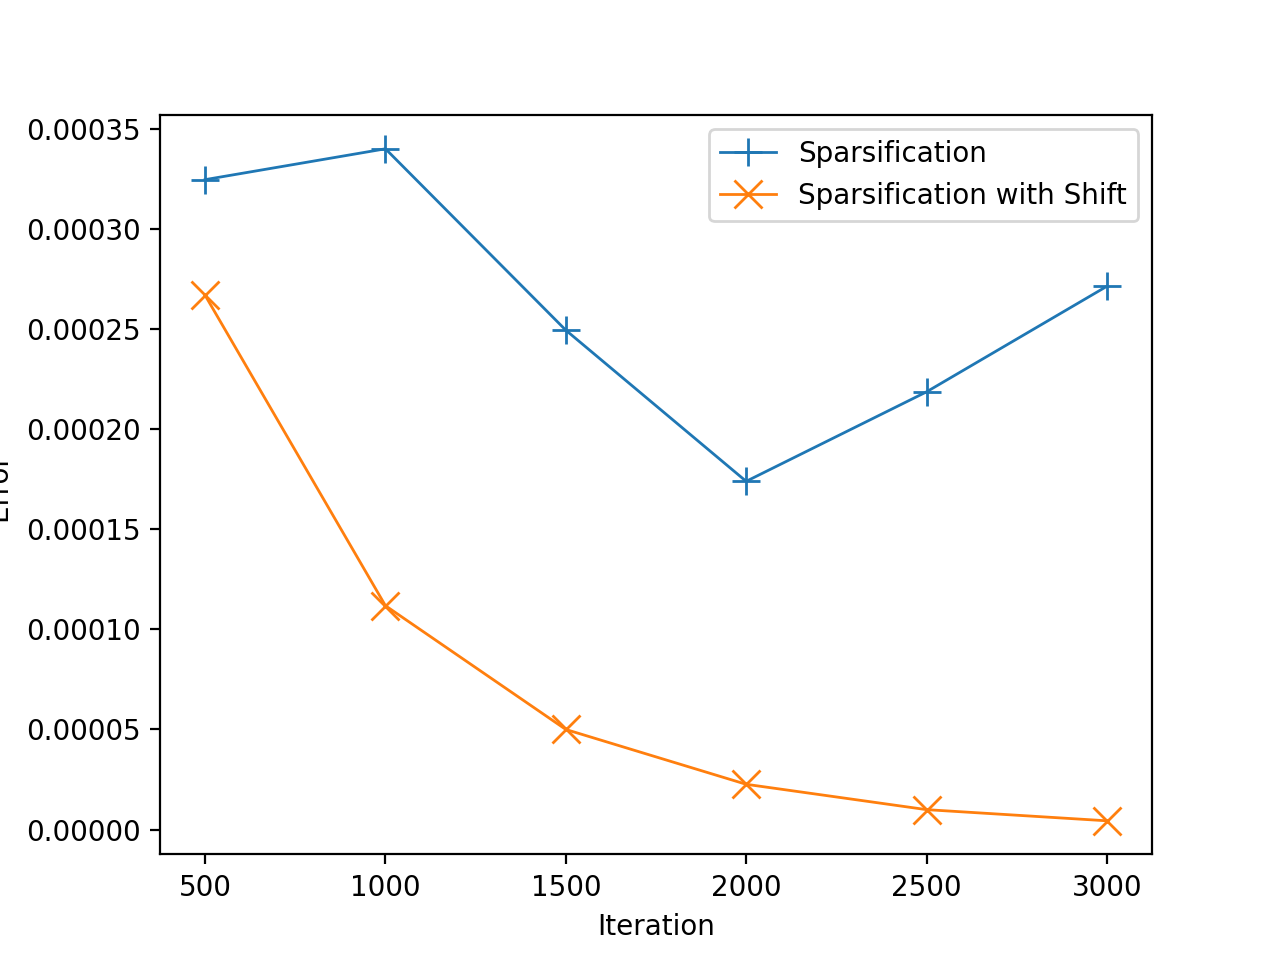
\includegraphics[width=6.7cm]{Figure_62.png}} 
	\subfigure[]{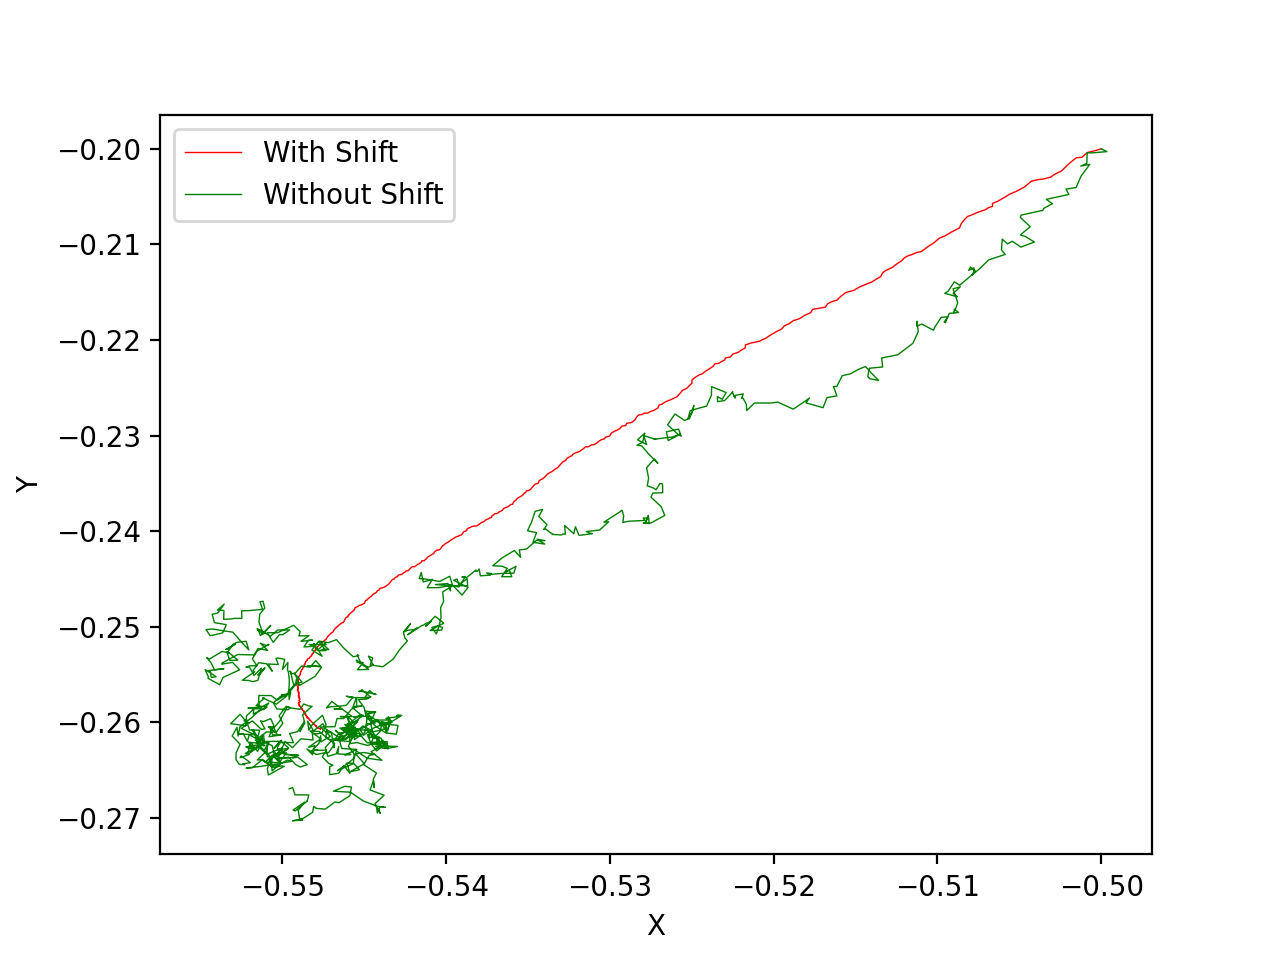
\includegraphics[width=6.7cm]{Figure_622.png}}
	\\ %换行
	
	
	\caption{ (a) shows the error in terms of iteration,(b) shows the trajectories of SGD-IND with shift and SGD-IND without shift} %图片标题
	\label{img1}
\end{figure}



\paragraph{p3.}
(1.) Since in this case 
$$
g^{k}=g\left(x^{k}\right)-g\left(y^{k}\right)+\nabla f\left(y^{k}\right)=\nabla f(x^k),
$$
which is exactly the descent direction for GD.
(2.)I don't find Corollary 95. Do you mean Corollary 97?
\begin{theorem}
	Assume $f$ is $\mu$-convex and L-smooth .The gradient estimator $g=\nabla f+\xi$ is unbiased and satisfies the expected smoothness bound
	$$
	\sigma(x) \stackrel{\text { def }}{=} \mathrm{E}\left[\left\|g(x)-g\left(x^{\star}\right)\right\|^{2}\right] \leq 2 L D_{f}\left(x, x^{\star}\right)
	$$
	Then L-SVRG with stepsize $\gamma=\frac{1}{6 L}$ satisfies
	$$
	\mathrm{E}\left[V^{k}\right] \leq\left(1-\min \left\{\frac{\mu}{6 L}, \frac{p}{2}\right\}\right)^{k} V^{0}
	$$
	where
	$$
	V^{k} \stackrel{(183)}{=}\left\|x^{k}-x^{\star}\right\|^{2}+M \gamma^{2} \sigma^{k}, \quad M=\frac{4}{p}, \quad \sigma^{k}=\sigma\left(y^{k}\right) \stackrel{\text { def }}{=} \mathrm{E}\left[\left\|g\left(y^{k}\right)-g\left(x^{\star}\right)\right\|^{2}\right]
	$$
	So,
	$$
	k \geq \max \left\{\frac{6 L}{\mu}, \frac{2}{p}\right\} \log \frac{1}{\varepsilon} \quad \Rightarrow \quad \mathrm{E}\left[V^{k}\right] \leq \varepsilon V^{0}
	$$
\end{theorem}
since $\max \left\{\frac{6 L}{\mu}, \frac{2}{p}\right\}>\frac{L}{\mu}$, so this kind of analysis is worse than GD. When p is not small, the order of convergence rate is the same between GD and L-SVRG($g=\nabla f+\xi$)(ignore the constant factor),  when p is small(like $p=\epsilon$), then the method in this problem is
much worse than GD. 
\paragraph{p4.}
The expected smoothness constant is $$
A^{\prime \prime}=\frac{n-\tau}{\tau(n-1)} \max _{i} L_{i}+\frac{n(\tau-1)}{\tau(n-1)} L
$$
In each iteration, one has to compute $2|S|=2\tau$ 1-gradient and p n-gradient,so
\begin{equation*}
	\textbf{COST}=2\tau +pn,
\end{equation*} 
so the total complexity is 
$$
\max\left\{\frac{6(\frac{n-\tau}{\tau(n-1)} \max _{i} L_{i}+\frac{n(\tau-1)}{\tau(n-1)} L)(2\tau+pn)}{\mu},\frac{2(2\tau+pn)}{p}\right\}\log(\frac{1}{\epsilon}),
$$
Computing the minimum point of $(\frac{n-\tau}{\tau(n-1)} \max _{i} L_{i}+\frac{n(\tau-1)}{\tau(n-1)} L)(2\tau+pn)$, it is $\tau_{\star}=\sqrt{\frac{(\max L_i-L)n^2p}{2(nL-\max L_i)}}$, since optimal $\tau$ should be an integer between 1 and n-1, we find optimal $\tau^{\star}$ between $\lfloor \tau_{\star}\rfloor$ and $\lceil \tau_{\star}\rceil$(only consider $\lfloor \tau_{\star}\rfloor,\lceil \tau_{\star}\rceil\in [1,n-1]$, if one of them is not in [1,n-1], ignore it), consider the $\hat{\tau}$, such that $\frac{6 A^{\prime\prime}}{\mu}=\frac{1}{p}$, if $\hat{\tau}>\tau^{\star}$, choose $\tau_{min}=\tau^{\star}$, else $\tau_{min}=optimal\{\lfloor\hat{\tau}\rfloor,\lceil\hat{\tau}\rceil\in \left[1,n-1\right]\}$. $\tau_{min}$ depends on p, if p is small, then $\tau_{min}$ is also small, if p is big, then $\tau_{min}$ will also get bigger.


\paragraph{p5.}


In my experiments(see Figure\ref{img2}.), I set $d = 2, n = 10,  f(x)=\frac{1}{ 10} \sum_{i=1}^{10} f_i(x), f_i(x) = \frac{1}{2}\left\|a_{i}^{} x-b_{i}\right\|_{2}^{2}$, $a = [matrix([[0.94884523, 0.31257516]]), matrix([[0.64695759, 0.79089169]]), \\matrix([[0.70218109, 0.91473775]]), matrix([[0.03035042, 0.21034799]]), \\matrix([[0.99278455, 0.2554682 ]]), matrix([[0.16064759, 0.09062056]]),\\ matrix([[0.41438167, 0.77718962]]), matrix([[0.4953842 , 0.93027311]]), \\matrix([[0.7692516 , 0.19772597]]), matrix([[0.12430258, 0.03779965]])],\\
b = [matrix([[0.4231786]]), matrix([[0.524466]]), matrix([[0.17981303]]), matrix([[0.50033184]]),\\ matrix([[0.71116473]]), matrix([[0.0604399]]), matrix([[0.37100656]]), matrix([[0.91263449]]),\\ matrix([[0.66417151]]), matrix([[0.65995097]])]
$, based on these information, we can get that $x_{\star} = matrix([[-0.54051746]
[-0.26890662]])$, I sample 10 points in the last step to estimate $\mathrm{E}\left[||x_{\text{last step}}-x_{\star}||^2\right]$.  The theory states that L-SVRG-NICE will converge to the optimal point while SGD-NICE will only converge to the neighborhood of the optimal point, this quite match the experiments results. You can see that the error of L-SVRG-NICE keeps dropping while SGD-NICE not and the trajectory of L-SVRG-NICE converge to the optimal point smoothly but the trajectory of SGD-NICE converges to the neighborhood of the optimal point with fluctuation.
\begin{figure}
	\centering
	\subfigure[ ]{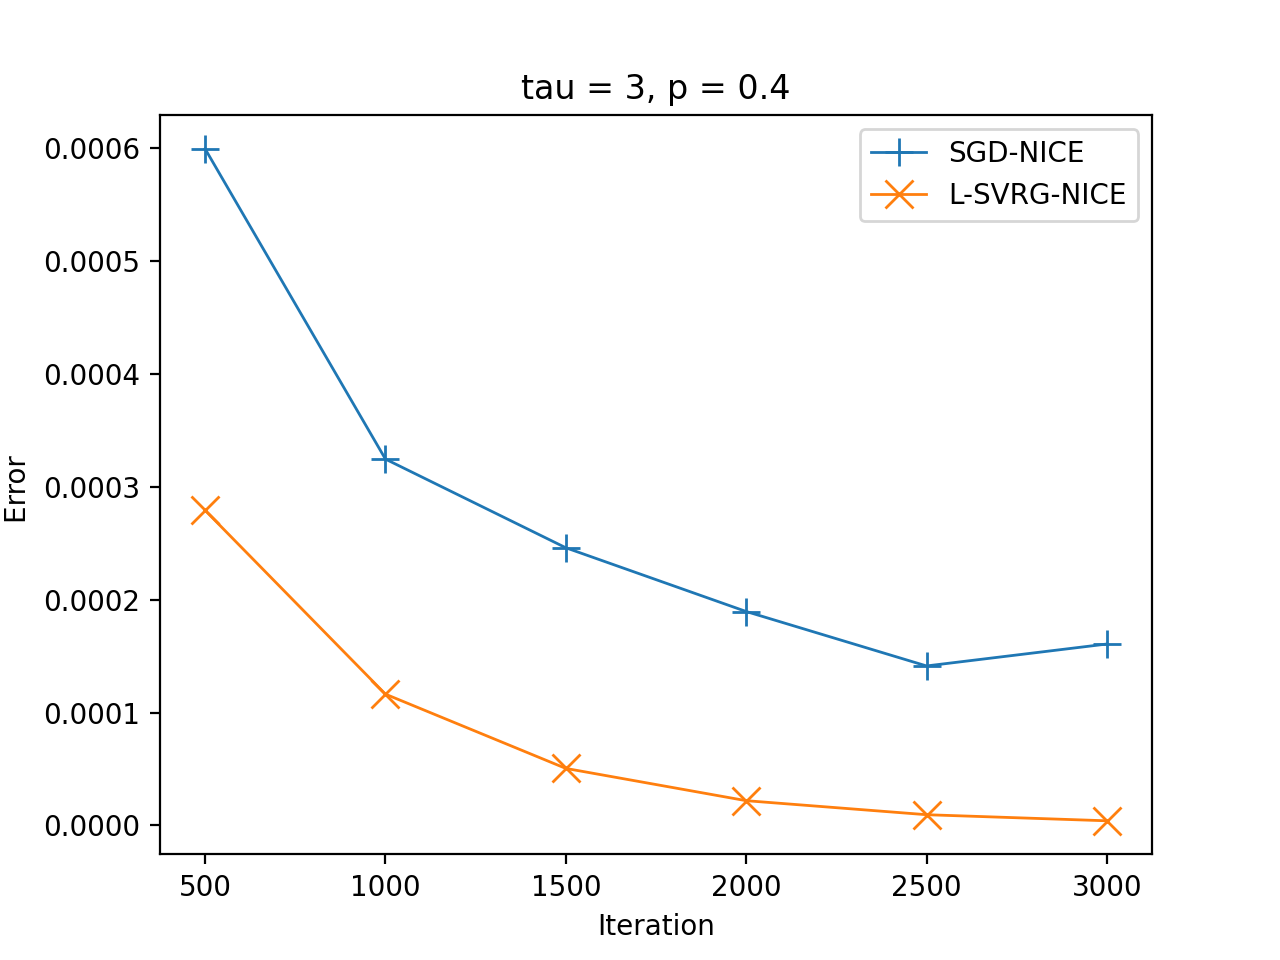
\includegraphics[width=6.7cm]{Figure_651.png}} 
	\subfigure[]{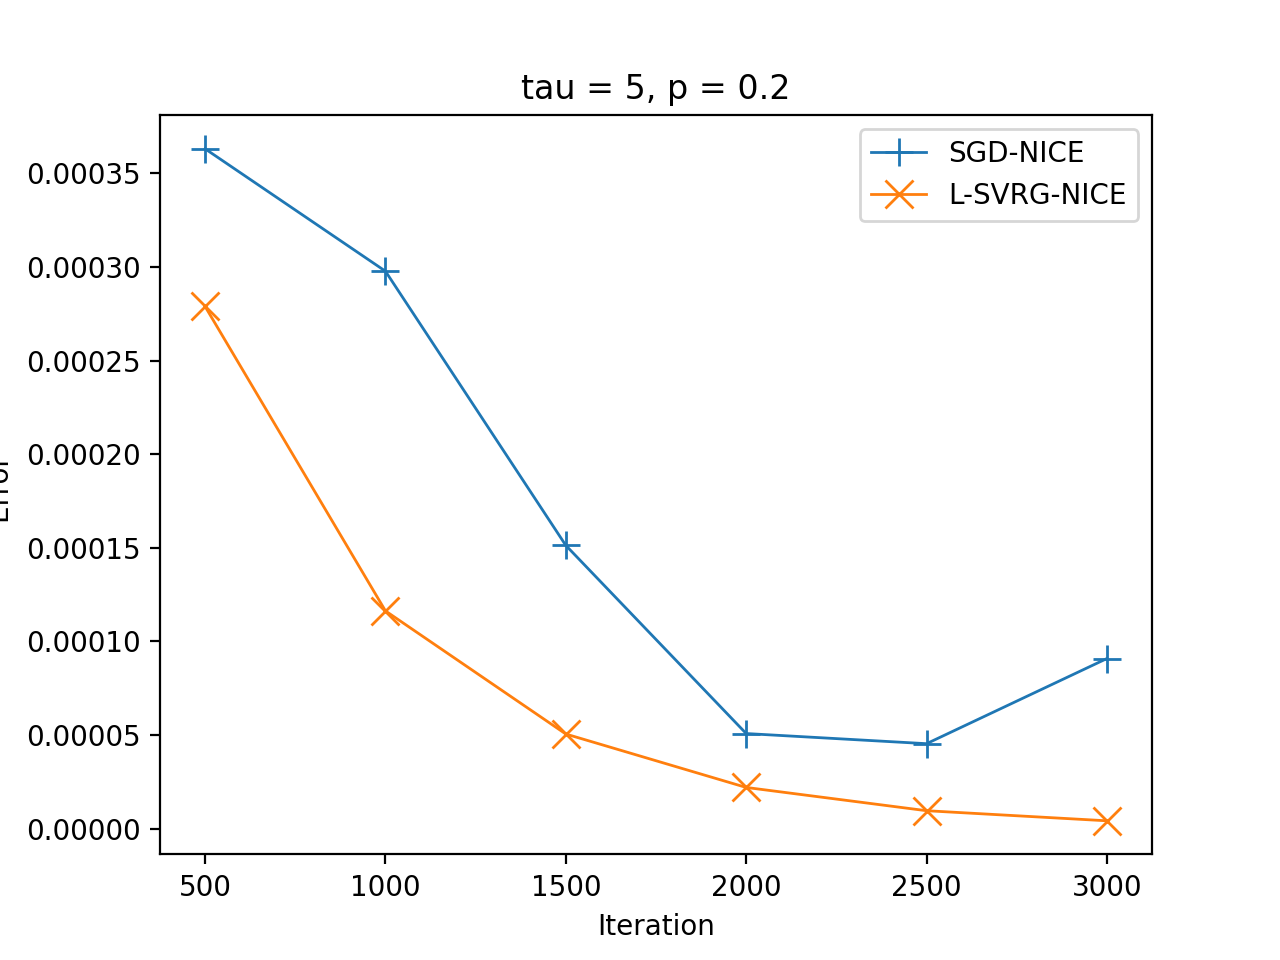
\includegraphics[width=6.7cm]{Figure_652.png}}
	\\ %换行
	\subfigure[ ]{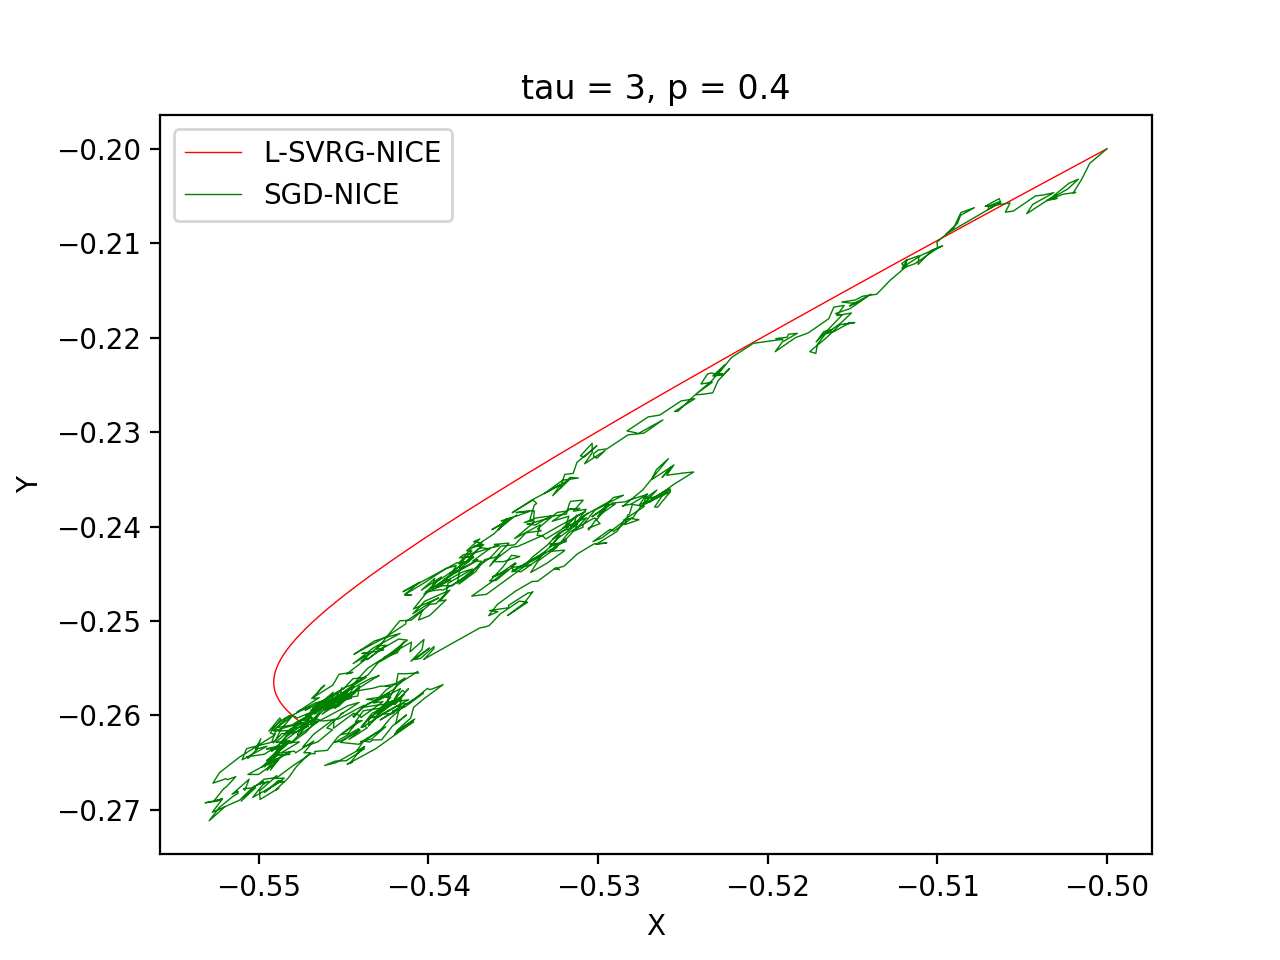
\includegraphics[width=6.7cm]{Figure_653.png}} 
	\subfigure[]{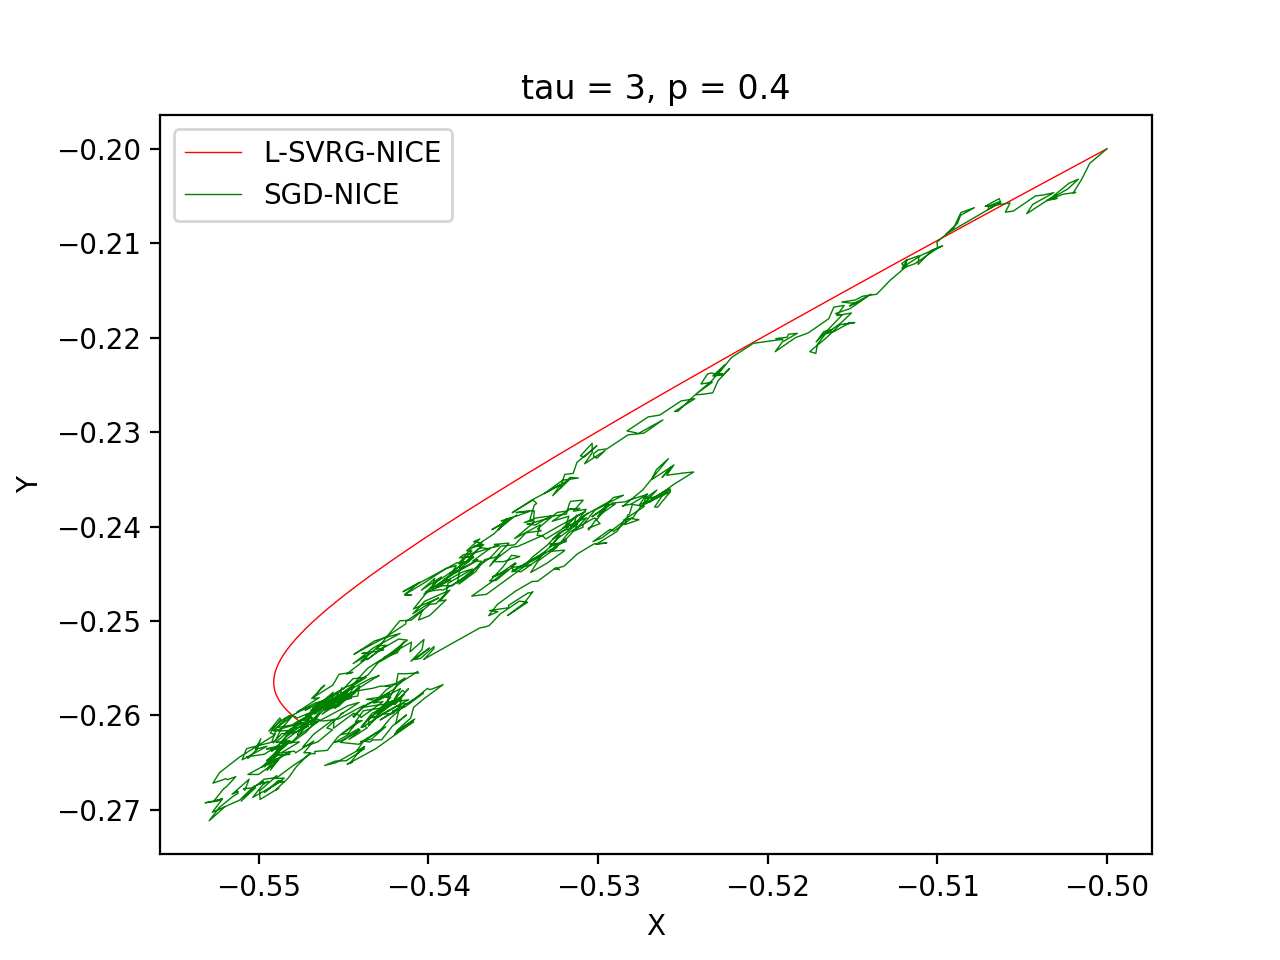
\includegraphics[width=6.7cm]{Figure_653.png}}
	
	
	\caption{ (a) shows the error in terms of iteration with $\tau = 3, p = 0.4$(b) shows the error in terms of iteration with $\tau = 5, p = 0.2$,(c)shows the trajectories of SGD-NICE and L-SVRG-NICE with $\tau = 3, p = 0.4$,(d) shows the trajectories of SGD-NICE and L-SVRG-NICE with $\tau = 5, p = 0.2$} %图片标题
	\label{img2}
\end{figure}



















	
\end{document}